\documentclass[abstract=on,9pt,twocolumn]{scrartcl}

\usepackage{ucs}
\usepackage[utf8x]{inputenc}
\usepackage[T1]{fontenc}
\usepackage[english]{babel}

%\usepackage{graphics}%	images other than eps

\usepackage[paper=a4paper,top=2cm,left=1.5cm,right=1.5cm,bottom=2cm,foot=1cm]{geometry}

\usepackage{relsize}%	relative font sizes

\usepackage[retainorgcmds]{IEEEtrantools}%	IEEEeqnarray
\setlength{\IEEEnormaljot}{4\IEEEnormaljot}

\usepackage{graphicx}
\usepackage{epstopdf}
\usepackage{indentfirst}
\usepackage{hyperref}
\usepackage{cleveref}
%\usepackage[noabbrev]{cleveref}
\usepackage{listings}
\usepackage{color}
\usepackage{todonotes}

%%%%%%%%%%%%%%%%
%  title page  %
%%%%%%%%%%%%%%%%
\titlehead{University of Minho \hfill Master's Degree in Informatics Engineering\\	Department of Informatics \hfill Parallel and Distributed Computing}

\title{A finite volume case study from an industrial application}

\subtitle{MPI: Implementation and Analysis}

\author{{\larger Group 1}\\Miguel Palhas \hfill--- \texttt{\smaller pg19808@alunos.uminho.pt}\\Pedro Costa \hfill--- \texttt{\smaller pg19830@alunos.uminho.pt}\\\smaller Stéphane Clain (co-Advisor)\\
}

\date{Braga, May 2012}

\subject{Integrated Project}


%%%%%%%%%%%
%  Hacks  %
%%%%%%%%%%%

%	Paragraph (title) with linebreak
\newcommand{\paragraphh}[1]{\paragraph{#1\hfill}\hfill

}

%	Add "Appendix" to the appendices titles, but not to the references
\usepackage{ifthen}
\newcommand*{\appendixmore}{%
  \renewcommand*{\othersectionlevelsformat}[1]{%
    \ifthenelse{\equal{##1}{section}}{\appendixname~}{}%
    \csname the##1\endcsname\autodot\enskip}
  \renewcommand*{\sectionmarkformat}{%
    \appendixname~\thesection\autodot\enskip}
}




\begin{document}
\maketitle

\begin{abstract}
This document presents a distributed memory implementation of the \texttt{polu} program using MPI and its analysis. The main problem of this implementation was partioning the mesh, which was solved using a naive approach. The resulting implementation presents clear speedups in the computational steps, but the results indicate that it is communication-bound. It presents good scalabilty in processors with a high amount of cores. The best results achieved are close to those of previous phases of this project, but the CUDA implementation stands out as the most promising for the final stage.
\end{abstract}
		% Abstract
\section{Introduction}
\label{sec:intro}

This document follows a previous work where \texttt{polu} application - which computes the evolution of a pollutant in a given environment - was studied in order to find possibilities of optimization and/or parallelization.

The original \texttt{polu} application works like a heartbeat algorithm with no communication (since it is executed in a single computation node). The algorithm used by the application sees the environment as a discrete mesh (represented by its cells and edges) and loops until the specified time interval is reached. At each iteration of this main loop, the algorithm performs two main steps:

\begin{description}
	\item[Flux Computation] Based on current pollution values for each cell, the flux for each edge is calculated (performed by the \texttt{compute\_flux} function)
	\item[Pollution Update] Using the previously calculated flux values, the pollution for each cell is updated (performed by the \texttt{update} function)
\end{description}

Several changes were performed in the original \texttt{polu} code in order to allow parallelization and/or improve performance. The most important of these optimizations involved changing the data structures (originally implemented as \textit{Arrays-of-Pointers}) to \textit{Arrays-of-Structures}. This change removed the excessive dereferencing caused by deep chains of pointers in the original structures, which effectively reduced data access time and improved locality.

The goal of this stage is to study attempt an implementation of the same application, using a distributed memory model with MPI, and analyze the scalability of the algorithm when testing with different amounts of processes and nodes.


\todo[inline]{Ate aqui esta copiado da intro do outro, com poucas alteraçoes}			% Introduction
\section{Mesh Partitioning}
\label{sec:partitioning}

The hardest task that needs to be done in order to allow a distributed memory implementation of the application is the partitioning of the data. The input consists solely of a two dimensional mesh, constituted by interconnected edges and cells. In each step, every edge and cell needs to access its neighbour cells or edges, respectively.

In order to distribute processing payload across each process, the input mesh, and all of the data associated with it, also needs to be distributed. A mesh partitioning algorithm is required. This algorithm must generate $P$ different partitions (where $P$ is the number of processors), each one corresponding to a subset of the original mesh. Each partition is then assigned to a single processor. Some aditional data is also required for each partition so that each process knows how it should communicate with the other partitions, so that the behavior can be simulated as if the mesh is being processed as a whole.

\subsection{Research in Mesh Partitioning}
\label{subsec:part_research}

Mesh partitioning is currently an actively researched topic, and some projects and libraries already exist that help with the understanding of how a mesh (or more generically, a graph) can be partitioned in ways to optimize certain aspects like load balancing, communication balancing or partitioning overhead. For instance, in \cite{metis}, a library called \texttt{Metis} is presented whose purpose is to solve this (and other) problems, by partitioning the mesh into $p$ partitions, roughly equal in size, such that the number of edges connecting multiple partitions is minimized. Other works found for this topic included \cite{gilbert1995,walshaw2000}.

However, given the time constraints of this project, and since the priority was to have a functional algorithm, it was decided not to attempt a mesh partitioning approach that would involve \textit{Metis} or any other researched work. Actually, the method used to partition the mesh is quite naive, as shown in \cref{subsec:part_method}

\subsection{Partitioning Methodology}
\label{subsec:part_method}

The algorithm created to partition the mesh works by dividing the input based on the centroid (the $(x, y)$ coordinates for the center point)) of each cell. Given a mesh with a total of 100 cells, and a pool of $P$ processes, it divides the mesh into $P$ partitions, each one with exactly $N=100/P$ cells, differing by at most one cell if they can't be divided evenly. To select which cells go to which process, the choice is based on the $x$ coordinate of each cell. They are first ordered into a set using $x$ as the ordering key, and then sequentially assigned to each process, in such a way that the first process receives the first $N$ cells of the set, the second process receives the next subset of size $N$, and so on until no more cells are left.

\begin{figure}[!htp]
	\begin{center}
		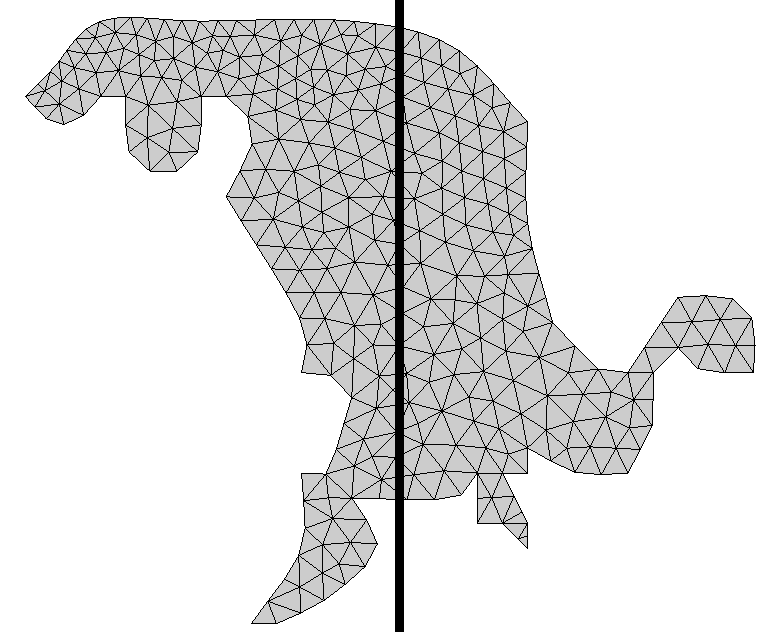
\includegraphics[width=\columnwidth]{report.may/images/foz_p2_msh}
	\end{center}
	\caption{Example of how the mesh will be partitioned when running the algorithm with 2 processes}
	\label{fig:tasktimeAOS}
\end{figure}

\begin{figure}[!htp]
	\begin{center}
		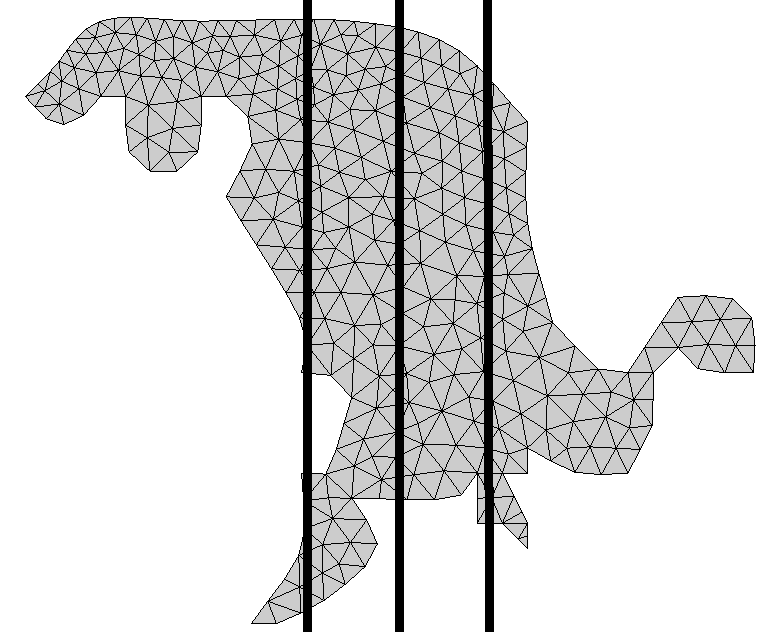
\includegraphics[width=\columnwidth]{report.may/images/foz_p4_msh}
	\end{center}
	\caption{Same example, but with 4 processes. Notice how the width of each partition is different, due the higher concentration of cells in the central area}
	\label{fig:tasktimeAOS}
\end{figure}

This sequential distribution, along with the need to sequentially order every cell of the mesh in order to distribute them, creates a rather large overhead in precomputational time.

After each cell is assigned, every partition then receives all the edges that are attached to their cells. At this point, some redundancy is created, as edges in the border of one partition will also exist in the neighbour partition.

Some preprocessing is also done at this stage, to index, for each partition, the subset of edges that connect to the left and right neighbours. Since the division is done vertically, by the $x$ coordinate of each cell, it is guaranteed that every partition will have at most two neighbours, one at the left side, and one at the right side (the only exception are the first and last partition which will only have one neighbour). It is also assumed that the width of the global mesh is big enough so that there are never any jumps between partitions, with a partition sharing an edge with another one which is not a direct neighbour of it.

This partitioning method, while guaranteeing that the load balancing is good in terms of amount of work per process, also suffers from not considering the size of the frontier of each partition, which will directly affect the size and overhead of the communication required between partitions.	% Partitioning
\section{MPI Implementation}
\label{sec:implementation}

\subsection{Data Structures}
\label{subsec:structs}

The first concern with a distributed memory implementation was the mesh partitioning process, which should be executed at the start of the program, guaranteeing that after it, each process will contain a local copy of a partition of the mesh, as well as the indexing structures that are necessary to describe how that partition connects with the rest of the mesh.

The partitioning process was already explained in \cref{sec:partitioning}. As for the indexing structures, they are generated while the partitioning process is being done.

First of all, when partitioning the mesh, if a given edge would be placed in the new border of the partition, with only its right cell existing, it should be swapped so that it is declared as its left cell. This was required, mostly for simplification process, as the whole \texttt{polu} has always had the assumption that the left cell always exist, and only the right cell should have the possibility of not existing, for the border edges. This is a common practice in Finite Volume Methods.

With that considered, the following indexing structures were required:
\begin{description}

	\item[\textbf\texttt{cell\_index}:] Stores, for each cell, the global index in the original mesh.
	\item[\textbf\texttt{edge\_index}:] Same as \texttt{cell\_index}, but for the edges.

	\item[\textbf\texttt{edge\_part}:] Can have the following values:
		\begin{description}
			\item[$0$:]  The right cell of this edge is in the same partition;
			\item[$-1$:] The right cell is in the left neighbor partition;
			\item[$1$:]  The right cell is in the right neighbor partition.
		\end{description}

	\item[\textbf\texttt{edge\_part\_index}:] For every edge with an \texttt{edge\_part} value of $-1$ or $1$, will give the corresponding index on the communication array that is received from either the left or right neighbor, according to which is connected to this edge.

	\item[\textbf\texttt{index\_to\_edge}:] Two arrays of this type exist for each partition, one for the left side and one for the right side. Unlike the previous ones, their size is equal to the size of the communication array instead of the total number of edges, and indicates for each value in the communication array, what is the corresponding edge that it refers to.

	\item[\textbf\texttt{cells\_send}:] Array used to send data to the neighbor partitions (one for the left, and one for the right)
	\item[\textbf\texttt{cells\_recv}:] Array used to receive data from the neighbors (one for the left, and one for the right)

\end{description}

\subsection{Communication Strategy}
\label{subsec:heartbeat_comm}

The original implementation iterates over two basic functions: \texttt{compute\_flux} and \texttt{update}, with each one iterating over all the cells and edges, respectively, and performing one of the steps of the heartbeat algorithm. To implement the required communication, an additional step was added to the beginning of the loop, calling the function \texttt{communication}, which copies the pollution data from the border cells to their corresponding locations on the communication array in each iteration. These arrays are then sent to their corresponding destinations, and the process then waits to receive the arrays that those neighbors also sent him.

After this step, the \texttt{compute\_flux} function is similar to the original function, with the exception that, when reading the pollution value for a right cell, it now has to check whether that right cell is stored in its own partition, or in a neighbor, in which case it will be required to read the value from the arrays received at the communication step. As for the \texttt{update} function, its implementation is exactly the same as the sequential version, since all the values for the flux of each edge are locally computed. There is, however, some redundancy here, as different partitions will compute the flux for the same edge, when this edge is located in the border between them.
% Implementation
\section{Results and Discussion}
\label{sec:results}

The environmental setup and a description of the methodology followed for these tests can be found in \cref{sec:environment,sec:methodology}.

The speedups achieved for each test performed on SeARCH Groups 101 and Hex are presented in \cref{fig:speedup}. Regarding the total execution, the MPI version achieves the best values without the Intel\textregistered Hyper-Threading Technology in the Group 101, and with it in Group Hex. Moreover, if one ignores the preparation phase (where the files are loaded and the mesh is partitioned), Intel\textregistered Hyper-Threading Technology allows for a linear speedup from the 24 processes test to the 48 processes test in Group Hex. For the bigger tests (48 and 96 processes in Groups 101 and Hex, respectively), when the number of processes exceeds the available hardware threads the results are worse (yet, in Group Hex this test is still better than the sequential version, which is not the case in Group 101). This is most probably explained by the process scheduling, which greatly affects communication by retaining in the queue one of the two processes communicating. Yet this was not further investigated.

\begin{figure}
	\begin{center}
		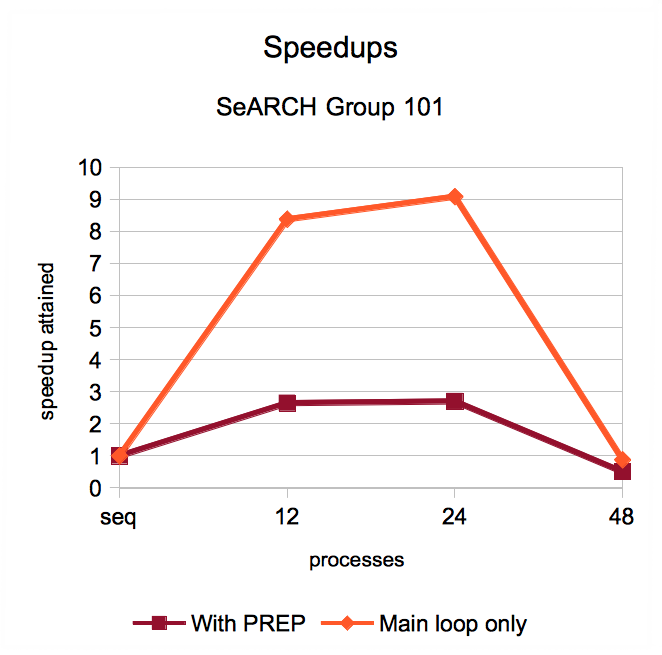
\includegraphics[width=\columnwidth]{report.may/images/speedup101.png}
		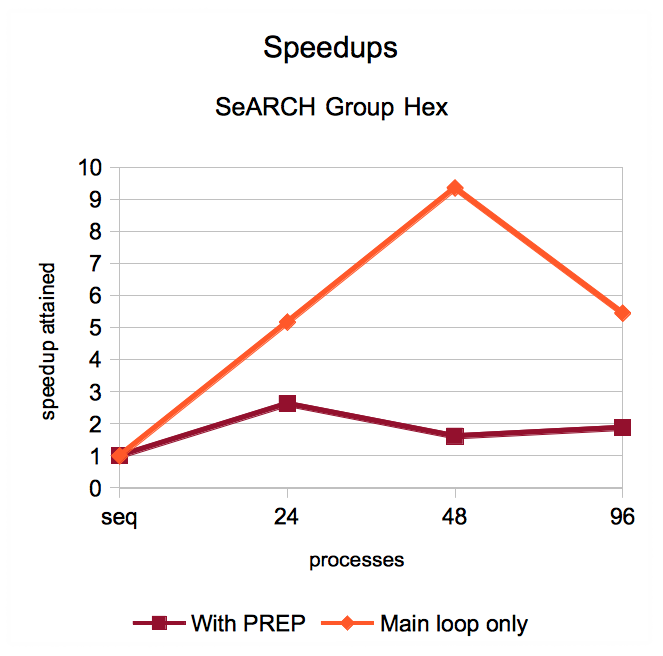
\includegraphics[width=\columnwidth]{report.may/images/speeduphex.png}
	\end{center}
	\caption[Speedups]{Speedups achieved for different numbers of processes on SeARCH Groups 101 and Hex.}
	\label{fig:speedup}
\end{figure}

Analyzing the execution times in \cref{fig:exectime}, one can easily spot the bottlenecks in each test (note the vertical axis, the execution time for the worst case in Group Hex is near the time for the best case in Group 101). For both groups, the sequential version presents the same picture: the update function takes most of the time due to the (already known from previous work) locality problems. For the MPI versions, the bottleneck of the entire execution is obviously the partitioning step, but since it is executed only once, its importance is diminished if the number of iterations is increased. Considering only the main loop, the communication tramples the other core functions, increasing when the number of processes is decreased (larger partitions mean that each inter-node communication holds more data) or increased beyond the hardware parallelism (as explained before, process scheduling hurts intra-node communication).

\begin{figure}
	\begin{center}
		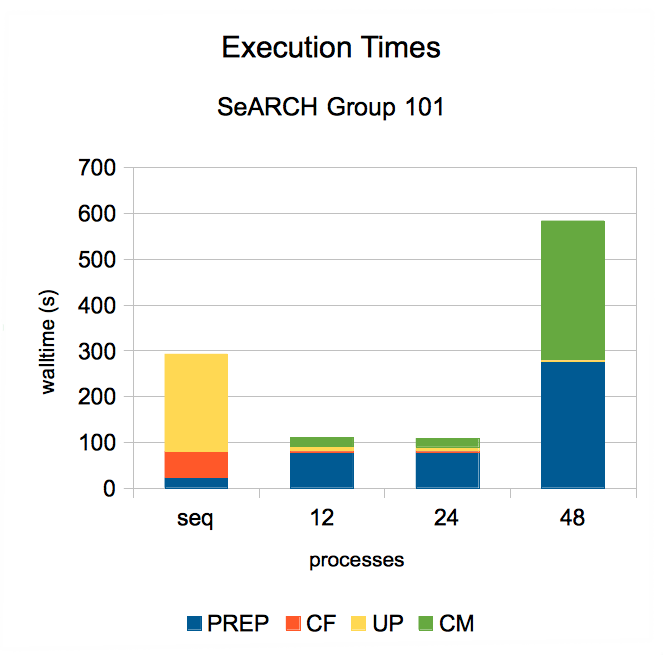
\includegraphics[width=\columnwidth]{report.may/images/exectime101.png}
		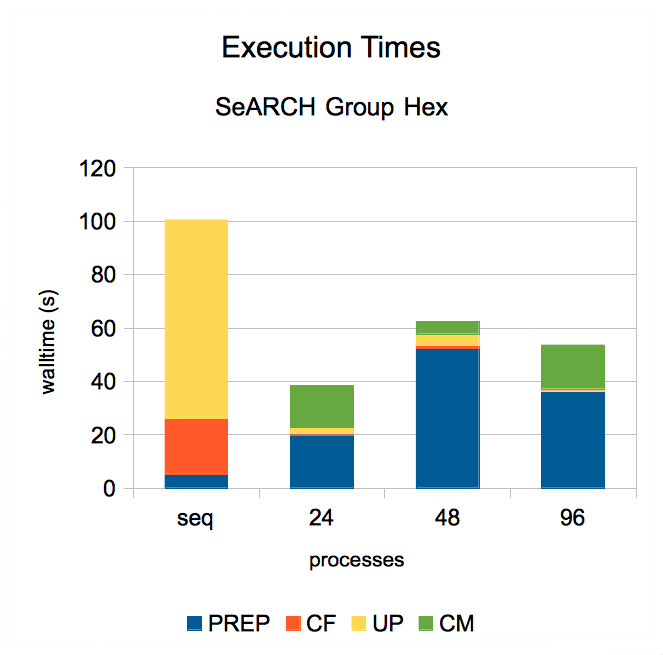
\includegraphics[width=\columnwidth]{report.may/images/exectimehex.png}
	\end{center}
	\caption[Execution times]{Execution times of the tests performed on SeARCH Groups 101 and Hex.}
	\label{fig:exectime}
\end{figure}

\Cref{fig:load1,fig:load2} show the distribution of work in a more obvious way. To note that the parallelism introduced reduces the \texttt{update} function from around 70\% to below 10\% (1\% for the bigger tests). Also noticeable is how the the preparation step and the communication domination change for different numbers of processes in the two node groups. In both groups, the introduction of Intel\textregistered Hyper-Threading Technology causes the partitioning process (memory-bound and mainly sequential, but with some parallelism) to be extended due to thread competition for resources. Then again, the increased number of processes causes partitions to be smaller, which reflects in a speedup in the communication step (very slight decrease in Group 101 but decreases to a fifth in Group Hex). Despite this, when the number of processes increases beyond the hardware available, as explained above the process scheduling will cause communication to take longer. In both Groups, this reflects in a very fast execution of \texttt{update} and \texttt{compute\_flux}, but 99\% of the whole program is spent in the preparation step and with communication.

\begin{figure*}[!p]
	\begin{center}
		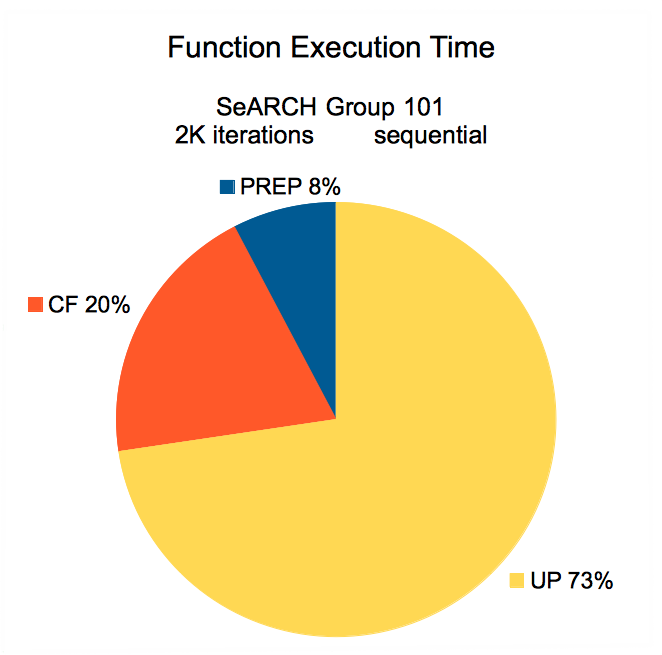
\includegraphics[width=\columnwidth]{report.may/images/loadseq101.png}
		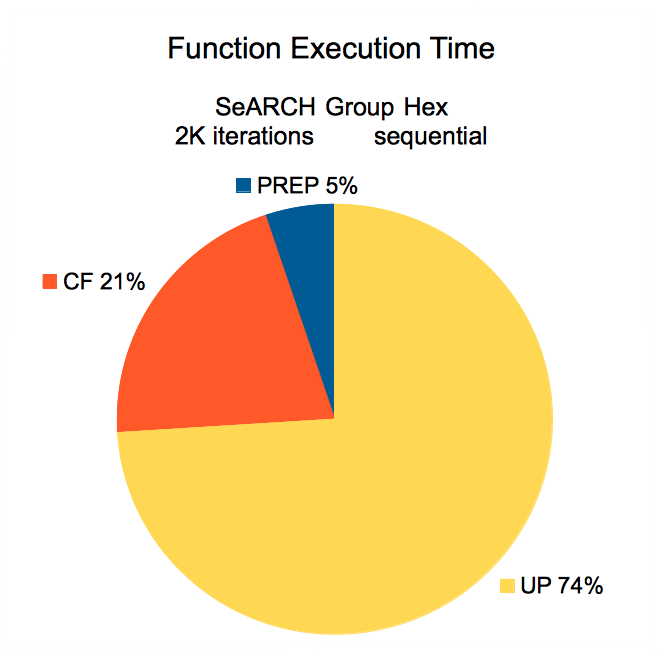
\includegraphics[width=\columnwidth]{report.may/images/loadseqhex.png}
		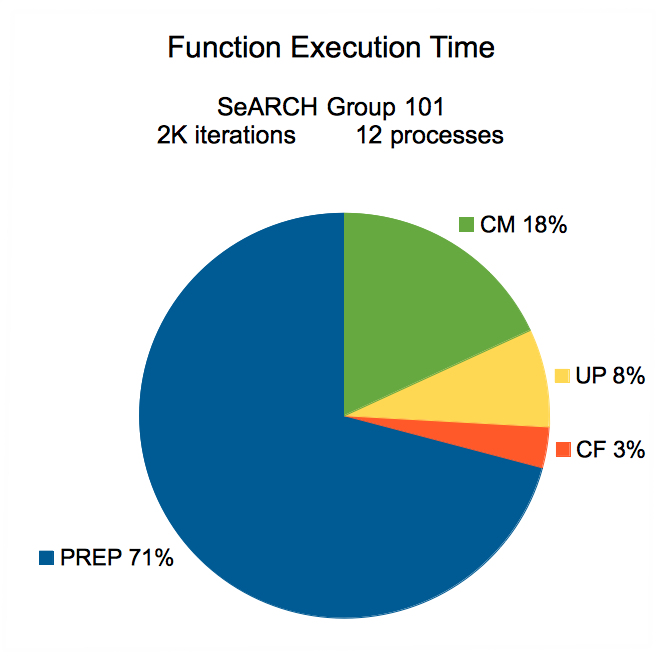
\includegraphics[width=\columnwidth]{report.may/images/load12101.png}
		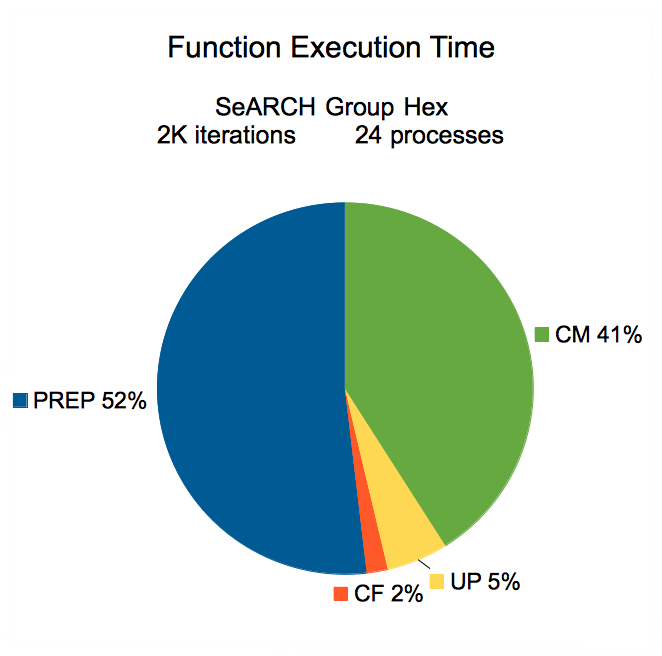
\includegraphics[width=\columnwidth]{report.may/images/load24hex.png}
	\end{center}
	\caption[Work loads]{Median work load of each part of the program in an execution, for the sequential version and the MPI version using half of the available hardware threads on SeARCH Groups 101 and Hex.}
	\label{fig:load1}
\end{figure*}

\begin{figure*}[!p]
	\begin{center}
		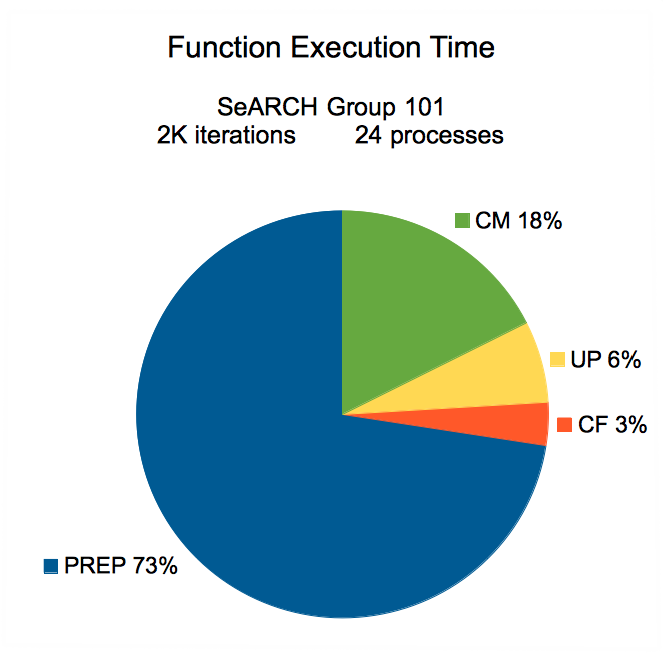
\includegraphics[width=\columnwidth]{report.may/images/load24101.png}
		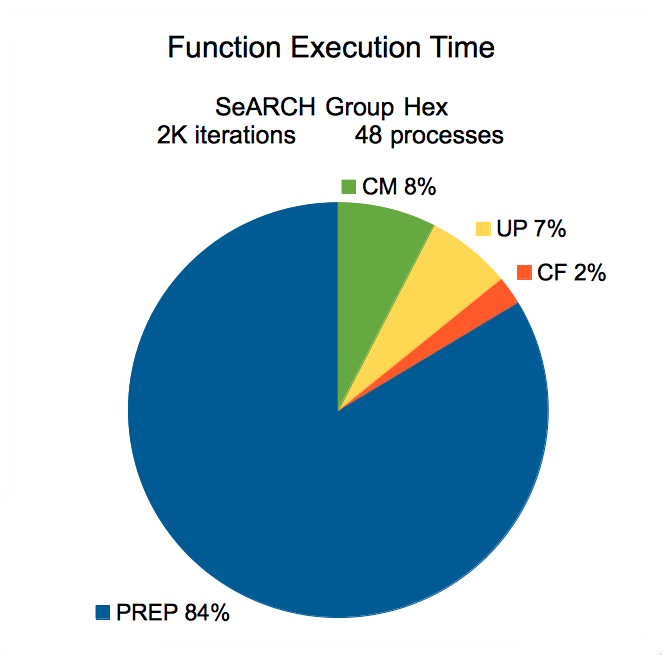
\includegraphics[width=\columnwidth]{report.may/images/load48hex.png}
		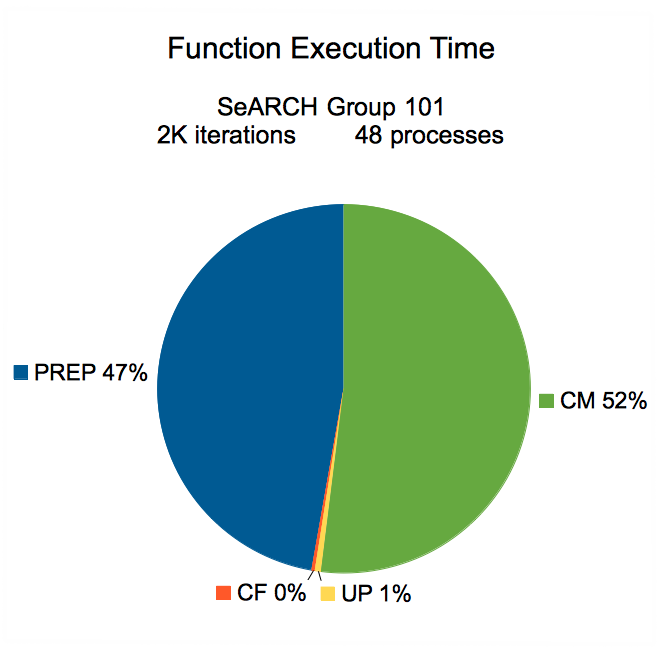
\includegraphics[width=\columnwidth]{report.may/images/load48101.png}
		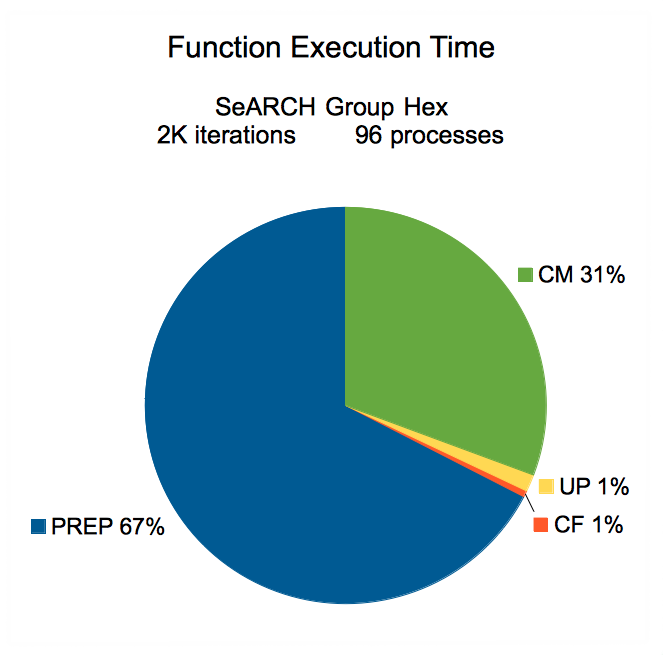
\includegraphics[width=\columnwidth]{report.may/images/load96hex.png}
	\end{center}
	\caption[Work loads]{Median work load of each part of the program in an execution, for the MPI version issuing processes in the exact number and the double of the available hardware threads on SeARCH Groups 101 and Hex.}
	\label{fig:load2}
\end{figure*}
		% Test Results
\section{Summary}
\label{sec:summary}

\Cref{tab:summary} shows a summary of all implemented versions of the algorithm so far. It should be highlighted that both the Environmental Setup and the testing Methodology differ between some tests. For instance. the initial tests, with the \textit{Original}, \textit{OpenMP AOS} and \textit{CUDA} implementations were performed using the SeARCH Group 511, and a full execution of the program (which, for the largest test case used, does around 20,000 iterations of the main loop).

The last two versions, \textit{OpenMP SOA} and \textit{MPI}, gave the best results on SeARCH Group Hex, and were only tested for a fixed amount of iterations, due to issues of availability of the nodes, which required a smaller amount of time to be requested. This approach depends on the homogeneity of the main loop (the workload does not change between iterations) and allows valid tests to be performed requiring only a fraction of the total time. Yet, since the amount of iterations is much smaller than the full execution would be, the impact of the preprocessing is much higher, especially in the MPI implementation, where the mesh partitioning introduces an even larger preprocessing time, when compared to the other versions.

\begin{table}[!htp]
		\smaller
		\begin{center}
			\begin{tabular}{l r ll}
			\hline
			\textbf{Implementation} & \textbf{\~ Time (s)}  & \textbf{Node Group}	& \textbf{Execution}	\\ \hline
			Original				& 6200				& 511				& Full							\\
			OpenMP AOS				& 1900				& 511				& Full							\\
			CUDA 					& 200				& 511 				& Full							\\ \hline
			OpenMP SOA 				& 36				& Hex 				& 1000 iter.					\\
			MPI 					& 38				& Hex 				& 2000 iter.					\\
			\hline
			\end{tabular}
		\end{center}
		\caption{Summary of all the \texttt{polu} versions implemented so far. Note that the environmental setup and methodology changed as the project evolved.}
		\label{tab:summary}
	\end{table}

Specially when taking into account the differences in the methodology, the CUDA implementation appears to be the one with the best performance gain. It is possible that the \textit{OpenMP SOA} and the \textit{MPI} implementations actually provide better execution times for a full execution, if it is considered that an amount of the time shown is spent in preprocessing. However, \cref{tab:summary} shows only the values for the best results, with the ``ideal'' number of processes and/or nodes. When the amount of processing units is increased, the speedups were shown not to be linear (see \cref{fig:speedup}).		% Summary of all implementations so far
\section{Conclusions}
\label{sec:conclusions}

\todo[inline]{Write this \ldots please \tiny{dumbass}}	% Conclusions

\bibliographystyle{IEEE}
\bibliography{report.mays}

\appendix

\section{Environmental Setup}
\label{sec:environment}

Two different types of nodes from the SeARCH cluster\footnote{\url{http://search.di.uminho.pt}} were used for the measurements reported in this document.

The nodes of the first type, referred to in this document as SeARCH Group 101, possess two single-core processors (with Intel\textregistered Hyper-Threading Technology) at a clock frequency of 3.2 GHz and 2 GB of RAM (see \cref{tab:group101}) for further detail regarding the hardware).

The second type -- SeARCH Group Hex -- contains nodes which have two hex-core processors (with Intel\textregistered Hyper-Threading Technology) and 12 to 48 GB of RAM (see \cref{tab:group601} for further details regarding this hardware).

The first group was used to perform tests using 6 fully reserved specific nodes\footnote{Some nodes in the SeARCH Group 101 showed odd behaviors. As such, the tests were limited to the six specially reserved nodes (21 to 26).}. As for the second group, the tests performed were limited to 2 non-specified nodes with a clock frequency of 2.66 GHz.

\begin{table}[!htp]
	\begin{center}
		\begin{tabular}{ll}
			\hline
			Processors per node: & 2	\\
			Processor model: & 64-bit Intel\textregistered Xeon\texttrademark	\\
			Cores per processor: & 1	\\
			Threads per core: & 2	\\
			Clock frequency: & 3.2 GHz	\\
			\hline
			L1 cache: & 16 KB (Data)	\\
			L2 cache: & 2 MB	\\
			L3 cache: & N/A	\\
			RAM: & 2 GB	\\
			\hline
		\end{tabular}
		\caption[SeARCH Group 101 hardware description]{SeARCH Group 101 hardware description. See \cite{xeon32} for further detail about this processor.}
		\label{tab:group101}
	\end{center}
\end{table}
	

\begin{table}[!htp]
	\begin{center}
		\begin{tabular}{lcc}
			\hline
			Processors per node: & 2	\\
			Processor model: & Intel\textregistered Xeon\textregistered X5650\\
			Cores per processor: & 6	\\
			Threads per core: & 2	\\
			Clock frequency: & 2.53 to 2.66 GHz	\\
			\hline
			L1 cache: & 32 KB + 32 KB per core	\\
			L2 cache: & 256 KB per core	\\
			L3 cache: & 12 MB shared	\\
			RAM: & 12 to 48 GB	\\
			\hline
		\end{tabular}
		\caption[SeARCH Group Hex hardware description]{SeARCH Group Hex hardware description. See \cite{xeon5600} for further detail about this processor.}
		\label{tab:grouphex}
	\end{center}
\end{table}
	% Test Env...
\section{Methodology}
\label{sec:methodology}

Only one kind of tests was performed with each version mentioned in this document, regarding execution time. Two timers were separatly measured: the first measured the total execution time, from the initialization of the MPI library to the respective finalization function; the second measured the execution time of each core function (\texttt{compute\_flux}, \texttt{update} and \texttt{communication}, except in the sequential version where no communication is performed). The main loop execution time is defined to be the sum of the times measured with the second timer, and aditional code to control the loop is neglected.

Several tests were performed for different numbers of processes with the MPI version. Using a fixed number of nodes (6 for SeARCH Group 101 and 2 for SeARCH Group Hex) and forcing the runtime tools to keep the load balanced between all the nodes, tests were performed for \texttt{2:1}, \texttt{1:1} and \texttt{1:2} (\texttt{processes:hardware threads}).

For each test 10 executions were performed (with 10 extra executions if the values presented high variation or were displaced) and the final results considered are the medians of the total values gathered by each timer.	% Test Method...

\end{document}
